\documentclass{article}
\usepackage[utf8]{inputenc}
\usepackage{physics}
\usepackage{listings}
\usepackage{graphicx}
\usepackage{flexisym}
\usepackage[export]{adjustbox}

%%%%%%%%%%%%%%%%%%%%%%%%%%%%%%%%%%
\documentclass[10pt, a4paper, twoside]{article}
\usepackage[margin=1in,bindingoffset=5.5mm,heightrounded]{geometry}
\usepackage[T1]{fontenc}
\usepackage{indentfirst}
%\vspace*{36 pt}
\title{Applied Mathematics TW324 Assignment 06}
\author{https://github.com/BhekimpiloNdhlela/TW324NumericalMethods \\ \\ Bhekimpilo Ndhlela (18998712)}
\date{11 May 2018}
\begin{document}
\maketitle
\pagebreak

\section*{Question 1}
\subsection*{Question 1a.)}
\textbf{\\Given: $y^{\prime \prime} +1001y\prime +1000y = 0$, and  $y(0) = 0, y\prime(1) = 0$ \\let: $y\prime = m$\\ therefore:\\ $m^2 + 1001m + 1000 = 0$\\ $(m + 1000)(m + 1) = 0$\\ $m_0 = -1000$ and $m_1 = -1$\\ therefore:\\ $y = c_1 e^{-1000t} + c_2e^{-t}$,   where $c_1$, $c_2$ $\in \mathbf{R}$\\ $y(0) = 0 = c_1 + c_2$\\ $y\prime(0) = 1 = -1000c_1 - c_2$\\
after solving these equations simultaneously for both $c_1$ and $c_2$ we get that \\
$c_1 =\frac{-1}{999}$ and $c_2 = \frac{1}{999}$ therefore the exact solution is:\\
$y(t) = \frac{-1}{999}e^{-1000t} + \frac{1}{999}e^{-t}$ Therefore I can conclude by stating that the problem is stiff}

\subsection*{Question 1b.)}
\textbf{\\$y^{\prime \prime} +1001y\prime +1000y = 0$ , $y(0) = 0, y\prime(1) = 0$ \\ Rewriting the equation above as a linear system of
the form: $\underline{\mathbf{y\prime}} = A\underline{\mathbf{y}}$\\ \\
From question 1a.) we know that:\\ $y(t) = \frac{-1}{999}e^{-1000t} + \frac{1}{999}e^{-t}$ \\
and therefore: \\  
$y\prime(t) = \frac{1000}{999}e^{-1000t} - \frac{1}{999}e^{-t}$ \\ therefore: \\ \\
$\underline{\mathbf{y\prime}}(t) $ = \begin{bmatrix}-1000 & 0\\ 0 & -1\\  \end{bmatrix}  \begin{bmatrix}\frac{-1}{999}e^{-1000t} \\
\frac{1}{999}e^{-t}\\ \end{bmatrix} \\ \\ let : $m_{1,_2} = \lambda_{1,2} = -1000, -1$ respctively \\ therefore: \\
$c = \mid \frac{min(\lambda_{1, 2})}{max(\lambda_{1, 2})} \mid = \mid \frac{-1000}{-1} \mid = 1000 \gg 1$ \\ \\
Therefore I can conclude by stating that the problem is stiff }

\subsection*{Question 1c.)}
\textbf{\\Since: $y^{\prime \prime} +1001y\prime +1000y = 0$\\ then: $\Rightarrow y^{\prime \prime} = - 1001y\prime -1000y$\\ \\ 
let:$v = y$ and $w = y\prime$ \\therefore: $v\prime = y\prime$ and $w\prime = y\prime\prime \Rightarrow$ $y\prime\prime= - 1001y\prime -1000y$ $ \Rightarrow y\prime\prime= - 1001w\prime -1000v$ \\
$v\prime = 0v + w$
$w\prime = -1000w - 1000v$\\ \\
therefore: \\
$\begin{bmatrix}v\prime\\ w\prime\\\end{bmatrix} = \begin{bmatrix}0 & 1\\ -1000 & -1001\\  \end{bmatrix} \begin{bmatrix}v\\w\\  \end{bmatrix}$ ,
where: \begin{bmatrix} v(0)\\ w(0) \\  \end{bmatrix} = \begin{bmatrix} 1\\ 0 \\  \end{bmatrix}}
\pagebreak

\subsection*{Python Source Code For Question 1c.)}
\begin{lstlisting}[language=Python]
def plot_solution_function(t_span, non_stiff_odes_s):
    plt.title("Solution Using A Non-Stiff ODE45 Method")
    plt.ylabel("y' = [dy1/dt ; dy2/dt]")
    non_stiff_t = linspace(t_span[0], t_span[1],\ 
                  len(non_stiff_odes_s[1]))
    plt.plot(non_stiff_t, non_stiff_odes_s[0,:], \ 
                  'k-', linewidth=4, label=" v' = w + 0v")
    plt.plot(non_stiff_t, non_stiff_odes_s[1,:],\ 
              'r-', linewidth=4, label=" w' = -1001w - 1000v")
    plt.legend(bbox_to_anchor=(.4, .4))
    plt.xlabel("time = t")
    plt.ylabel("y' = [dy1/dt ; dy2/dt]")
    plt.show()

if __name__ == "__main__":
    from numpy import linspace, array, shape
    import matplotlib.pyplot as plt
    from scipy.integrate import solve_ivp

    y0     = [1., 0.]
    t_span = [0., 1.]
    f      = lambda t, y: array([y[0], -1001*y[0] -1000*y[1]])

    non_stiff_odes = solve_ivp(f, t_span, y0, method='RK45')
    plot_solution_function(t_span, non_stiff_odes.y)
\end{lstlisting}
\begin{figure}[h!]
  \centering
  \begin{subfigure}{\linewidth}
    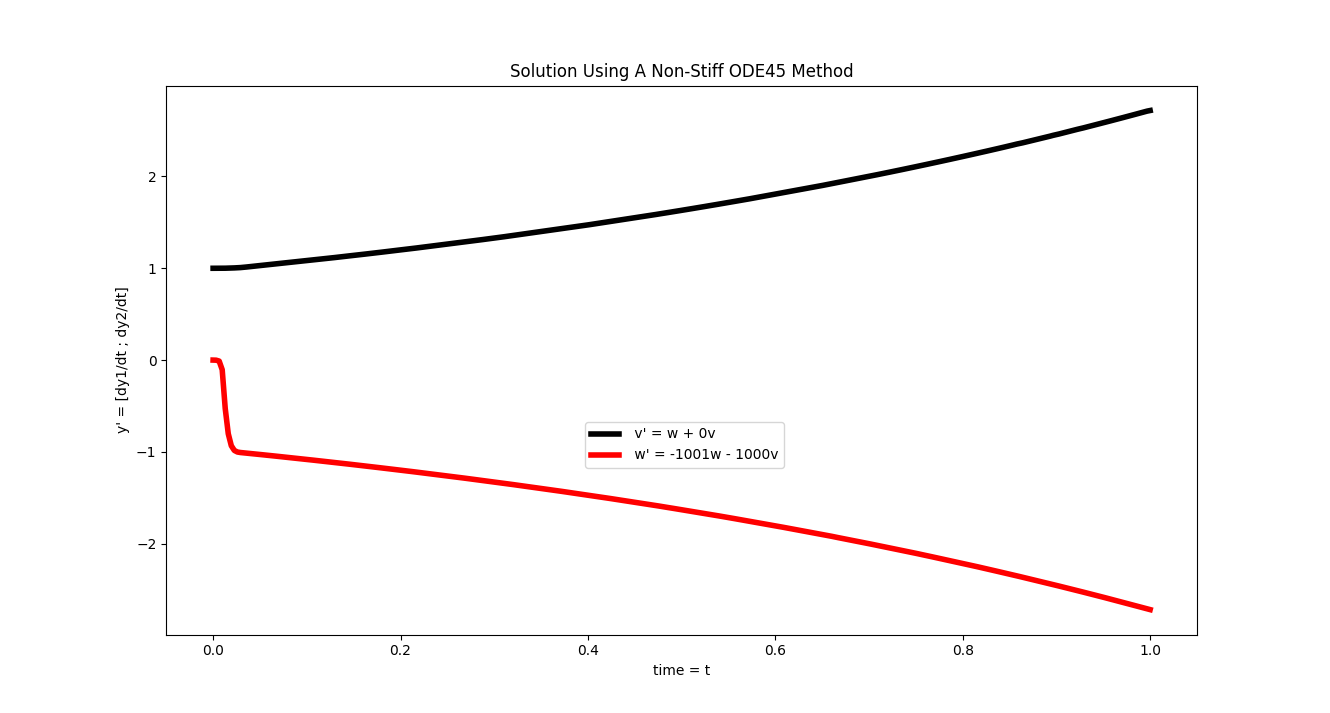
\includegraphics[width=\linewidth]{q1c.png}
    \caption{Numerically Solution Using RK45}
  \end{subfigure}
\end{figure}
\pagebreak


\subsection*{Python Source Code For Question 1d.)}
\begin{lstlisting}[language=Python]
def plot_solution_functions(t_span, non_stiff_odes_s, stiff_odes_s):
    plt.subplot(211)
    plt.title("Solution Using A Non-Stiff ODE Method")
    plt.ylabel("y' = [dy1/dt ; dy2/dt]")
    non_stiff_t = linspace(t_span[0], t_span[1], len(non_stiff_odes_s[1]))
    plt.plot(non_stiff_t, non_stiff_odes_s[0,:], 'k-',\ 
                          linewidth=4, label=" v' = w + 0v")
    plt.plot(non_stiff_t, non_stiff_odes_s[1,:], 'r-',\ 
                          linewidth=4, label=" w' = -1001w - 1000v")
    plt.legend(bbox_to_anchor=(.4, .4))
    plt.subplot(212)
    plt.title("Solution Using A Stiff ODE Method")
    plt.xlabel("time = t")
    plt.ylabel("y' = [dy1/dt ; dy2/dt]")
    stiff_t = linspace(t_span[0], t_span[1], len(stiff_odes_s[1]))
    plt.plot(stiff_t, stiff_odes_s[0,:], 'k-', \ 
             linewidth=4, label=" v' = w + 0v")
    plt.plot(stiff_t, stiff_odes_s[1,:], 'r-', \ 
             linewidth=4, label=" w' = -1001w - 1000v")
    plt.show()

def plot_time_comparisons(t_span, non_stiff_odes_t, stiff_odes_t):
    plt.subplot(211)
    non_stiff_t = linspace(t_span[0], t_span[1], len(non_stiff_odes_t))
    plt.ylabel("Time Steps")
    plt.title("Method of Non-Stiff odes(RK45) = "+\ 
               str(len(non_stiff_t)) + " Steps.")
    plt.plot(non_stiff_t, non_stiff_odes_t, 'k-', linewidth=4)
    plt.subplot(212)
    plt.xlabel("Time = t")
    plt.ylabel("Time Steps")
    stiff_t = linspace(t_span[0], t_span[1], len(stiff_odes_t))
    plt.title("Method of Stiff ODEs(BDF) = "+ str(len(stiff_t)) + " Steps.")
    plt.plot(stiff_t, stiff_odes_t, 'r-', linewidth=4)
    plt.show()

if __name__ == "__main__":
    from numpy import linspace, array, shape
    import matplotlib.pyplot as plt
    from scipy.integrate import solve_ivp

    y0     = [1., 0.]
    t_span = [0., 1.]
    f      = lambda t, y: array([y[0], -1001*y[0] -1000*y[1]])

    non_stiff_odes = solve_ivp(f, t_span, y0, method='RK45')
    stiff_odes     = solve_ivp(f, t_span, y0, method='BDF')

    plot_solution_functions(t_span, non_stiff_odes.y, stiff_odes.y)
    plot_time_comparisons(t_span, non_stiff_odes.t,  stiff_odes.t)
\end{lstlisting}
\subsection*{Solution and Time Comparison Curves For Question 1d.)}
\begin{figure}[h!]
  \centering
  \begin{subfigure}{\linewidth}
    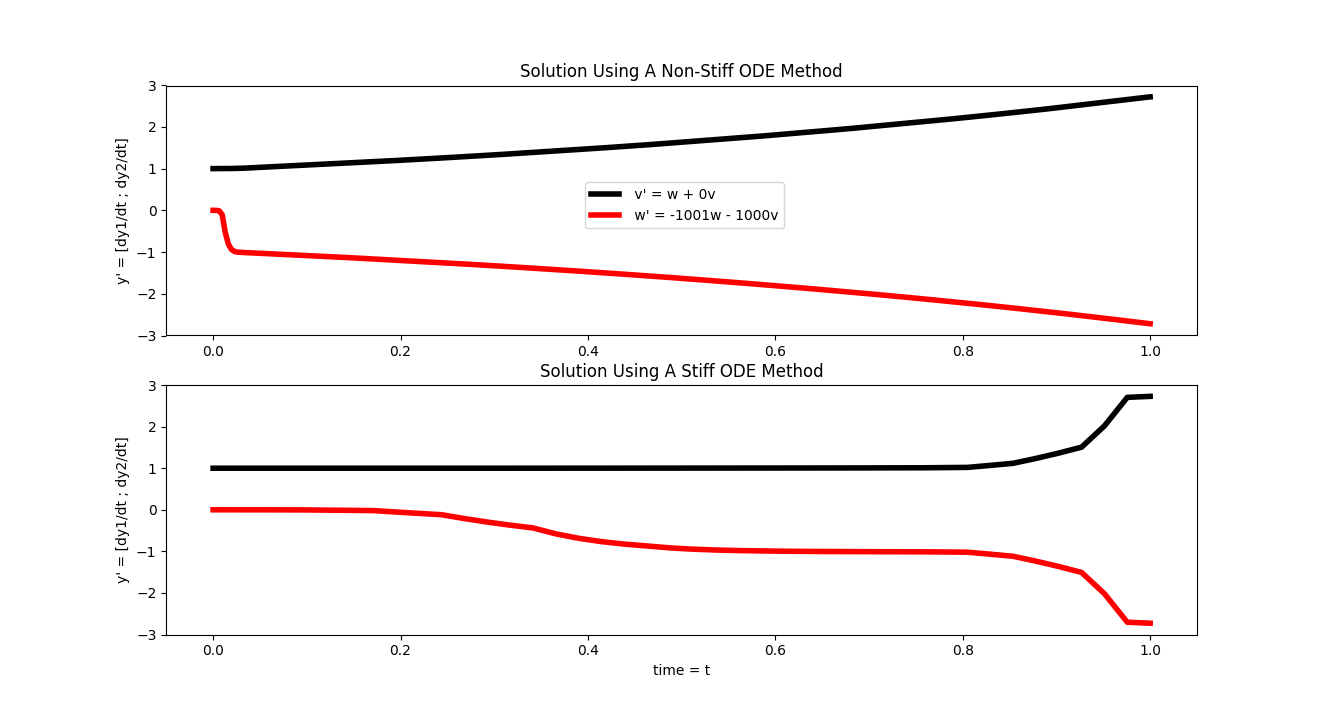
\includegraphics[width=\linewidth]{q1_sol.png}
    \caption{Solution Curve Comparisons, between the Non-Stiff and Stiff methods of ODEs}
  \end{subfigure}
\end{figure}
\begin{figure}[h!]
  \centering
  \begin{subfigure}{\linewidth}
    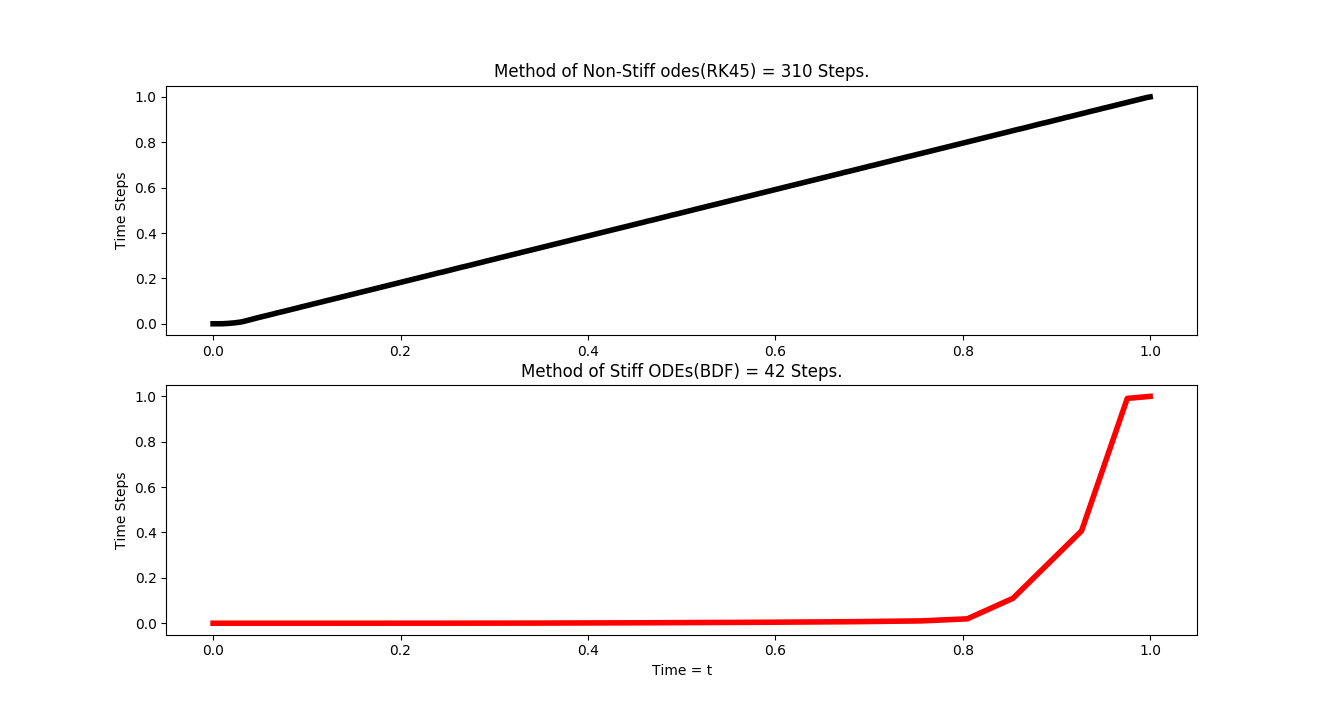
\includegraphics[width=\linewidth]{q1_t_comp.png}
    \caption{Time Curve Comparisons, between the Non-Stiff and Stiff methods of Solving ODEs}
  \end{subfigure}
\end{figure}


\pagebreak
\section*{Question 2}
\subsection*{Question 2a.)}
\begin{lstlisting}[language=Python]
# RK stages
s1 = f(t, yn)
s2 = f(t + h, yn + h * s1)
s3 = f(t + h/2.0, yn + (h/4.0)*(s1 + s2))
p  = 3
yn1 = yn + (h/6.0)*(s1 + 4.0*s3 + s2)
# Error estimate
err = h/3.0 * abs(s1 - 2.0*s3 + s2)           
\end{lstlisting}
\subsection*{Question 2b.)}
\begin{lstlisting}[language=Python]
if __name__ == "__main__":
    import numpy as np
    import numpy.linalg as npla
    import matplotlib.pyplot as plt
    
    # making use of ODE23
    tt, yy = ode23(lambda t, y: y**2 - y**3, [0, 2.0/0.001], y0=0.001)
    plot_functions(tt, yy)
\end{lstlisting}

\begin{figure}[h!]
  \centering
  \begin{subfigure}{\linewidth}
    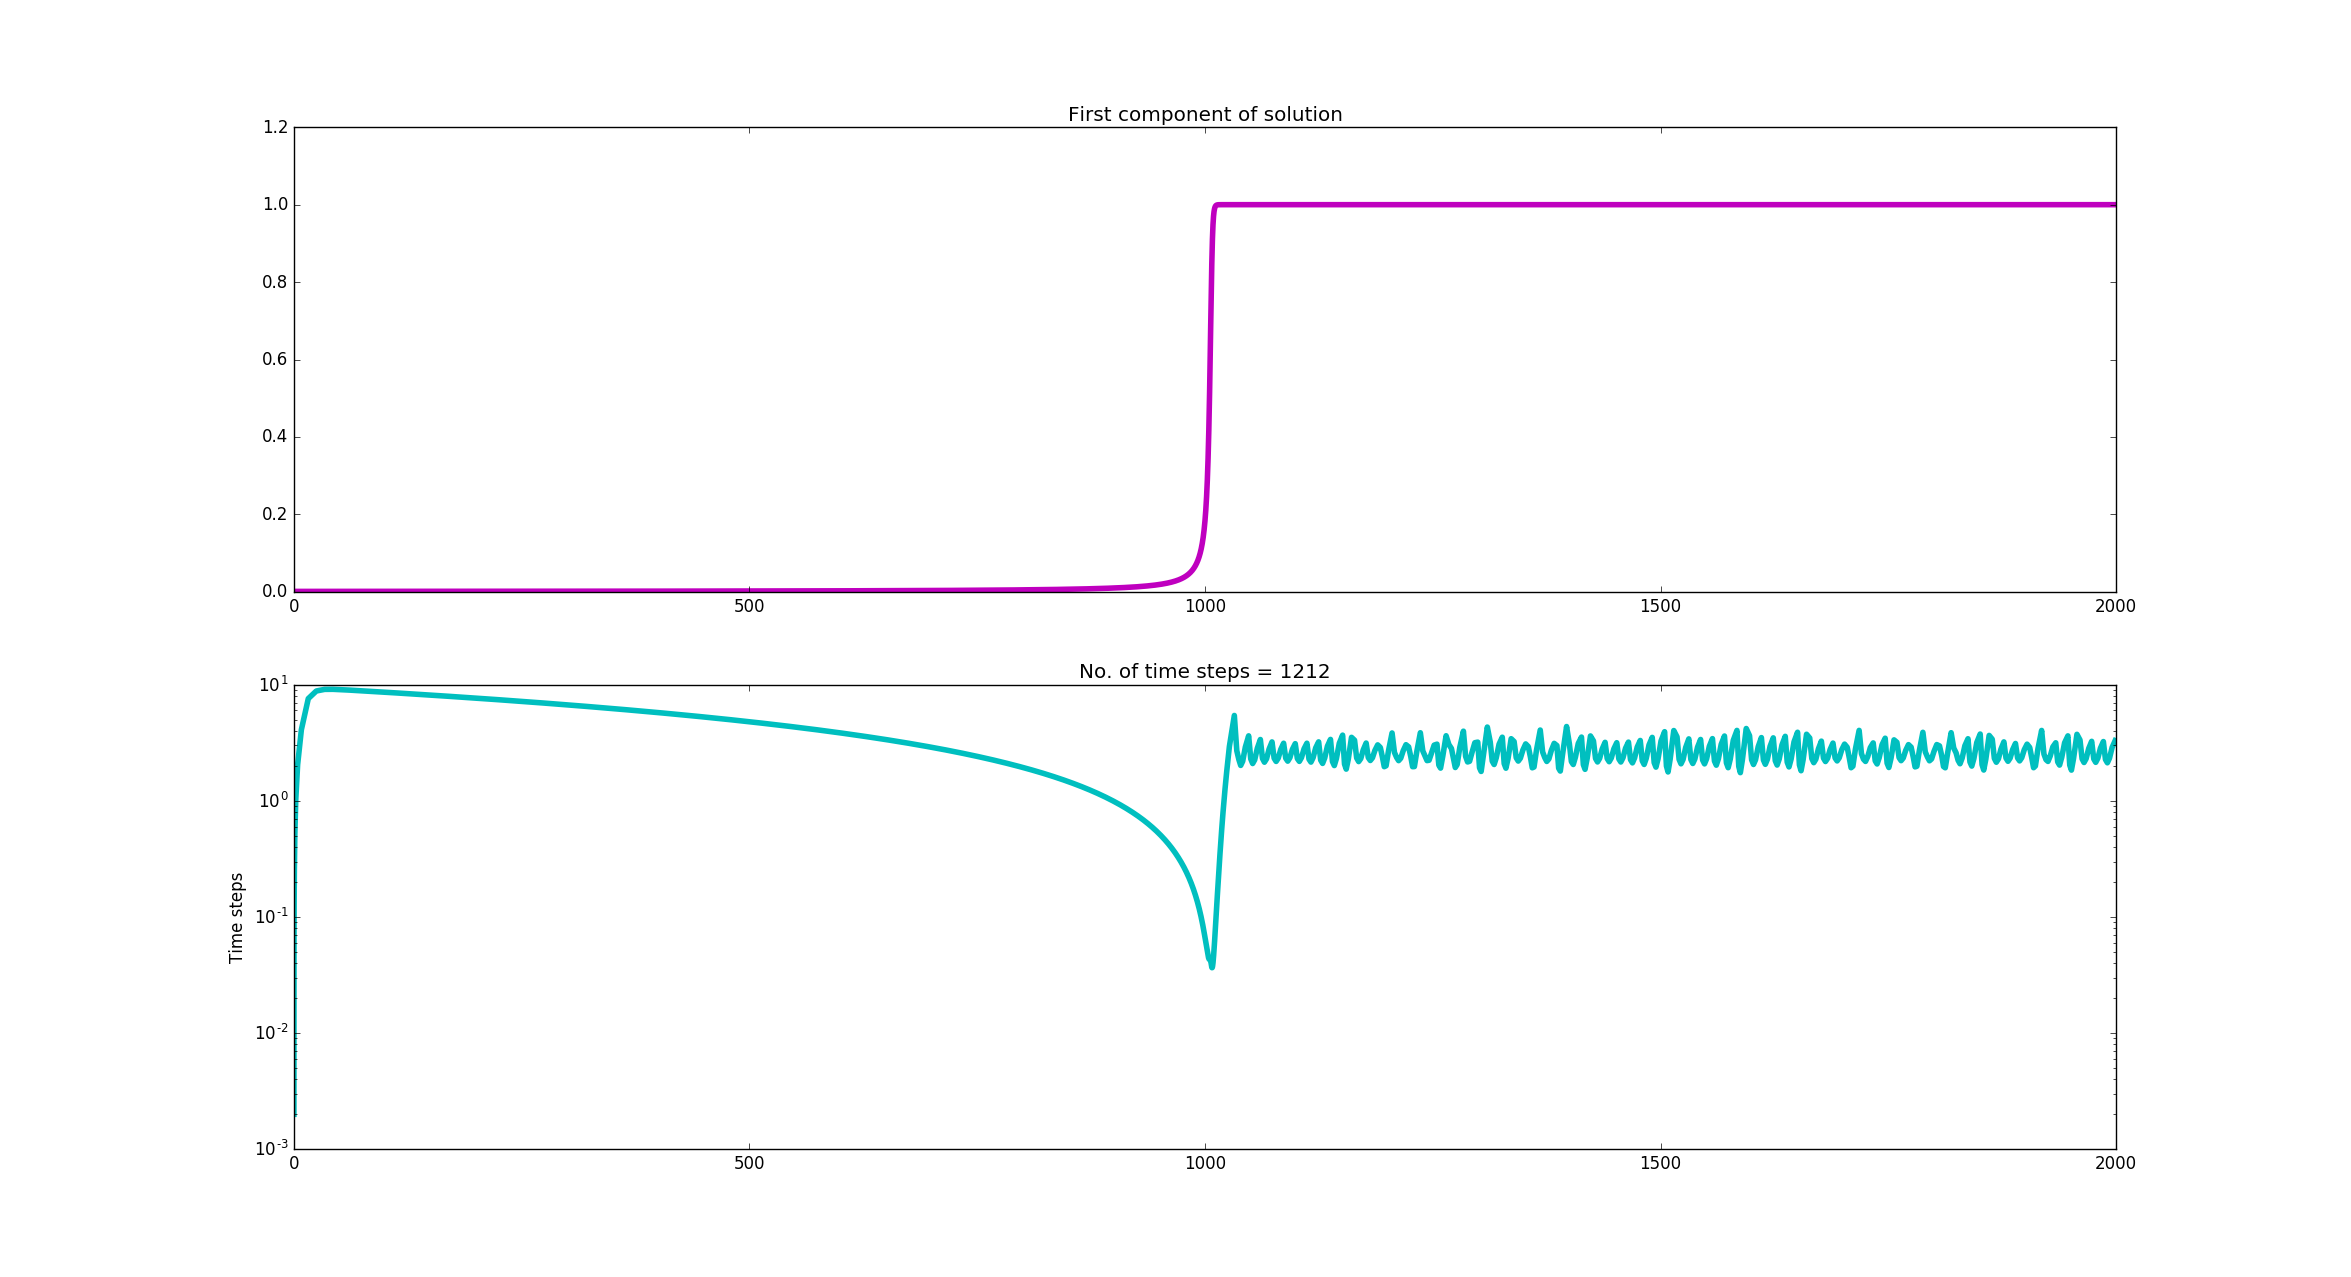
\includegraphics[width=\linewidth]{q2a.png}
    \caption{Approximation using ode324}
  \end{subfigure}
\end{figure}
\pagebreak
\subsection*{Question 2c.)}
\begin{lstlisting}[language=Python]
# RK stages
s1 = f(t, yn)
s2 = f(t + (0.25)*h, yn + (0.25)*h * s1)
s3 = f(t + (3./8.)*h, yn + (3./32.)*h*s1 + (9./32.)*h*s2)
s4 = f(t + (12./13.)* h, yn + (1932./2197)*h*s1 - \
     (7200./2197.)*h*s2 + (7296./2197.)*h*s3)
s5 = f(t + h, yn  + (439./216.)*h*s1 - 8.0*h*s2 + \
     (3680./513.)*h*s3 - (845./4104.)*h*s4)
s6 = f(t + .5 * h, yn - (8./27.)*h*s1 + 2.0*h*s2 - \
     (3544./2565.)*h*s3 + (1859.0/4104.0)*h*s4 - (11./40.)*h*s5)
p  = 5;
yn1 = yn + h*((16.0/135.0)*s1 + (6656.0/12825.0)*s3 +\
     (28561.0/56430.0)*s4 - (9.0/50.)*s5 + (2./55.)*s6) ;
# Error estimate
err = h * abs((1.0/360.0)*s1 - (128.0/4275.0)*s3 - \
      (2197.0/75240.0)*s4 + (1.0/50.0)*s5 + (2.0/55.0)*s6) ;
\end{lstlisting}

\subsection*{ Python Client Source Code For the ode45 function}
\begin{lstlisting}[language=Python]
if __name__ == "__main__":
    import numpy as np
    import numpy.linalg as npla
    import matplotlib.pyplot as plt

    # making use of ODE45
    tt, yy = ode45(lambda t, y: y**2 - y**3, [0, 2.0/0.001], y0=0.001)
    plot_functions(tt, yy)
\end{lstlisting}
\begin{figure}[h!]
  \centering
  \begin{subfigure}{\linewidth}
    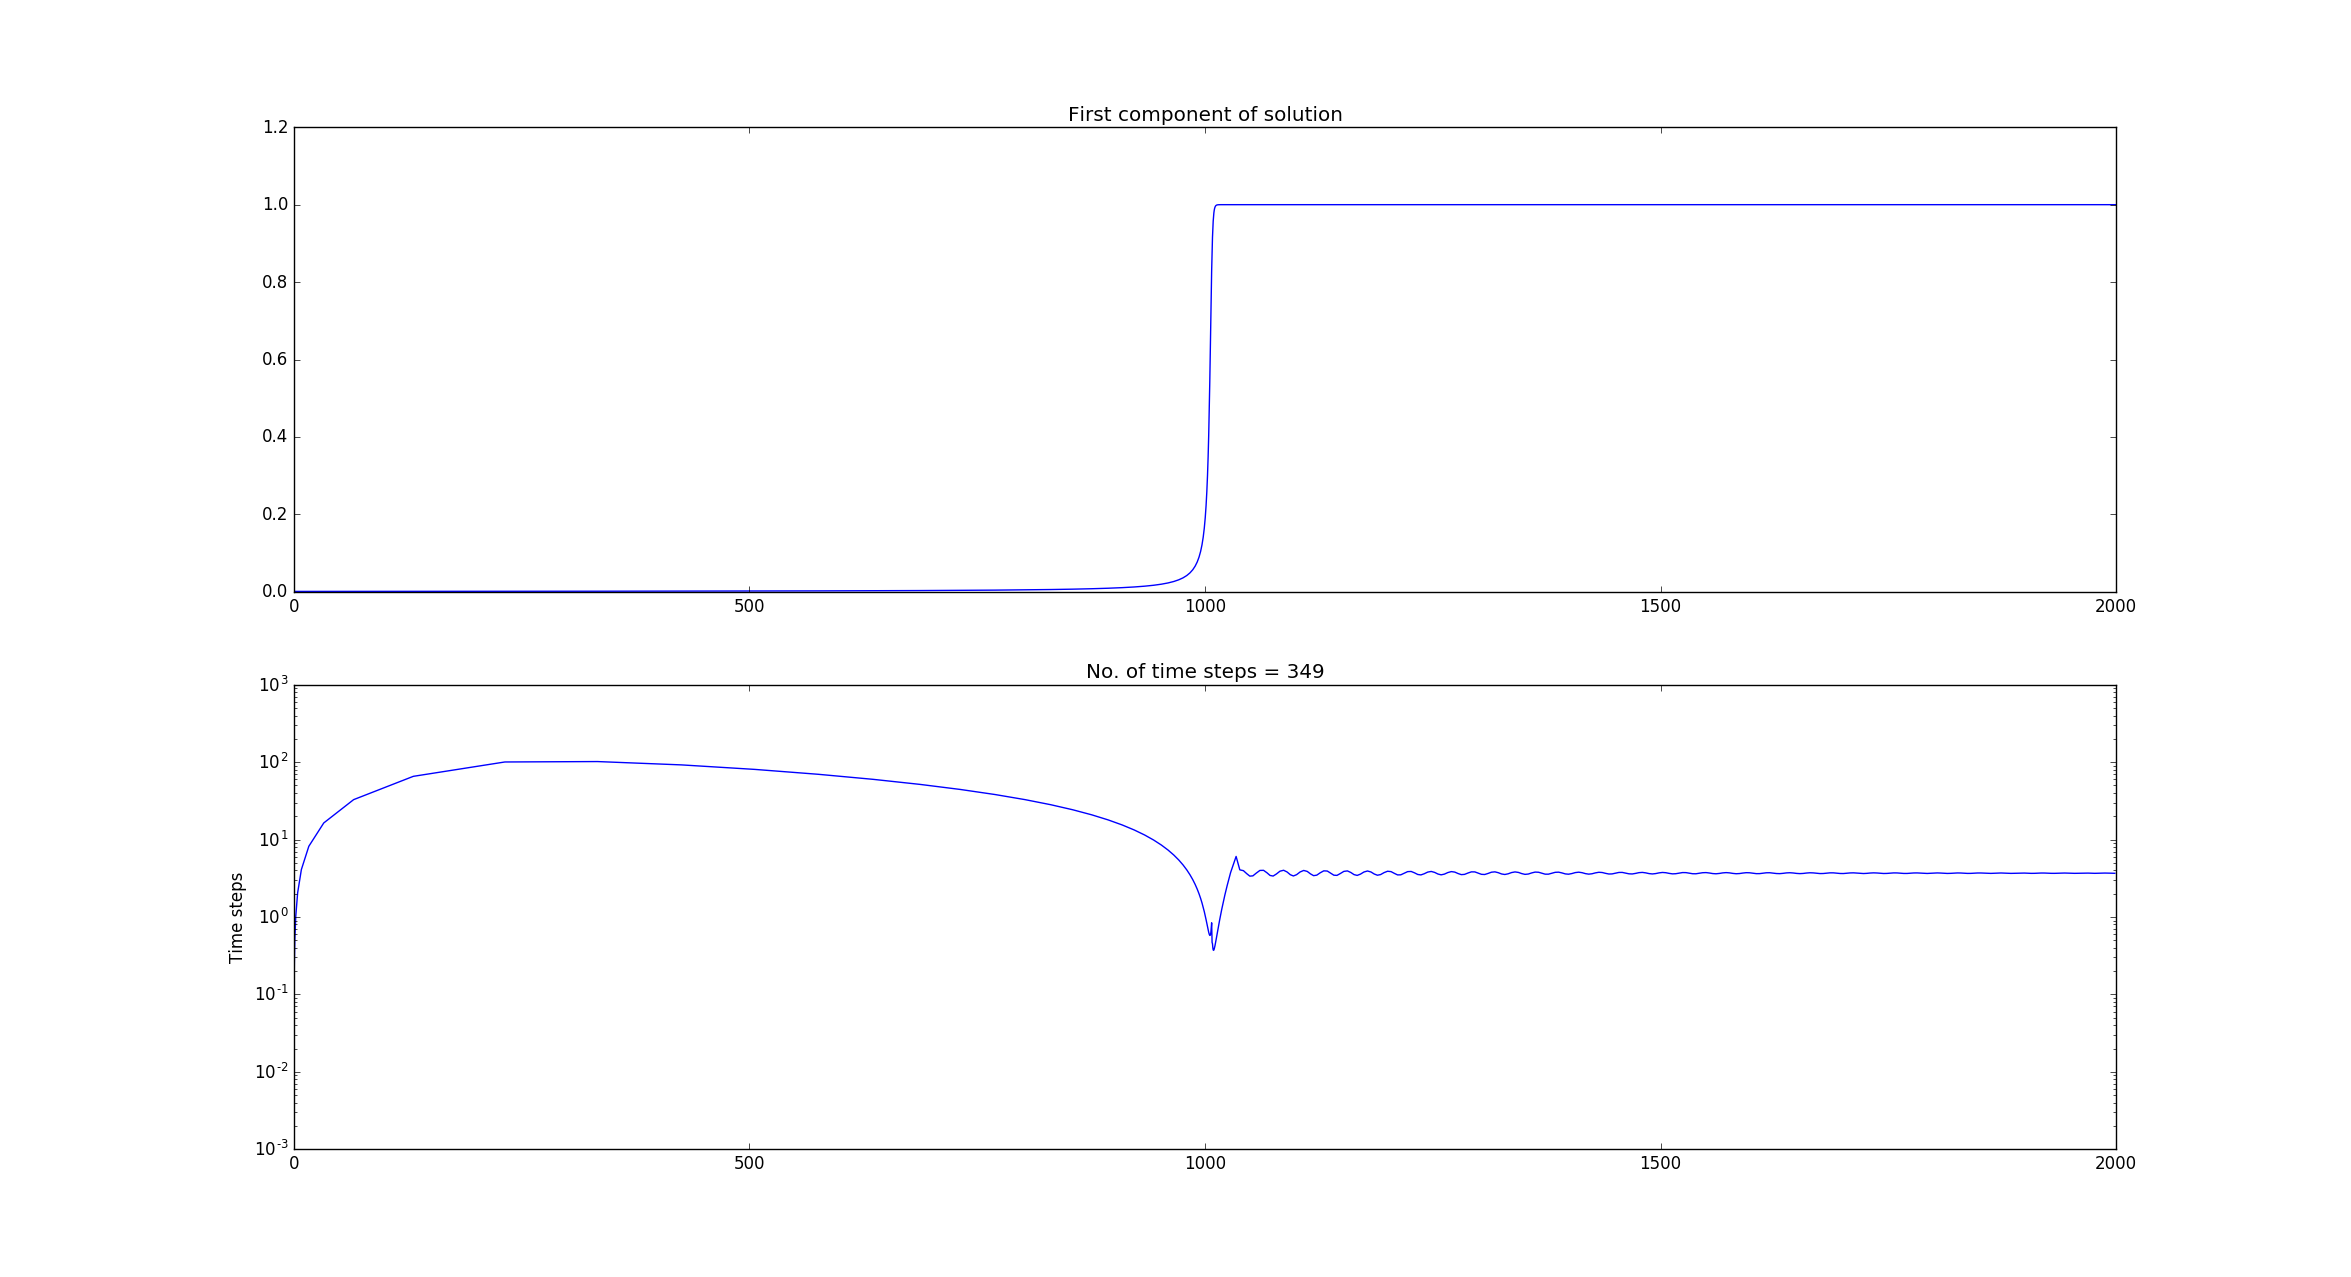
\includegraphics[width=\linewidth]{q2c.png}
    \caption{Approximation using RK45}
  \end{subfigure}
\end{figure}

\textbf{\\ \\ \\The famous RKF45 pair with $p = 5$ proves to be more efficient compared to the approach ode324 which implements the embedded Explicit Trapezium and Simpson pair with $p = 3$ and $z_{i+1}$, this becomes evident if one compares the number of time steps it take to solve or converge to the First component of the solution. since the RK45 takes $348$ time steps compared to $1212$ time steps that were achieved by the ode324.}
\pagebreak

\section*{ Question 3}
\subsection*{Python Source Code For Question 3a.) }
\begin{lstlisting}[language=Python]
def adam_bashforth_two_step(f, n, h, t=[1.0, 2.0], w0=4.0):
    W    = zeros((int(n),), dtype=float)
    t    = linspace(t[0], t[1], int(n))
    W[0] = w0
    W[1] = W[0] + h * f(t[0], W[0])    # w[1] evaluated by euler's method
    for i in range(1, int(n - 1)):
        W[i+1] = W[i] + (0.5*h)*(3*f(t[i], W[i]) - f(t[i-1], W[i-1]))
    return W[-1]

def debug(H, N, AE, W, debug_status=True):
    if debug_status == True:
        print("Adam BashForth Two(2) Step Algorithm")
        print("H \t N  \t\tAbs_Err \t W[-1] approx @ t=2")
        for h, n, ae, w in zip(H, N, AE, W):
            print n, "\t{:.4f}\t".format(h), "\t{:.15f}".format(ae),\ 
                  "\t{:.15f}".format(w)
            
from numpy import (exp, zeros, linspace)
import matplotlib.pyplot as plt

f       = lambda t, y : -t * y
I       = 4.0*exp(0.5*(1-((2)**2.0)))
N       = [100.0, 200.0, 400.0]
H       = [1/ N[0], 1/N[1], 1/N[2]]

# do for the Adam Bashforth two step Method
w_ad2s  = [adam_bashforth_two_step(f, n, h) for n, h in zip(N, H)]
ae_ad2s = [abs(w - I) for w in w_ad2s]
debug(H, N, ae_ad2s, w_ad2s)
\end{lstlisting}
\textbf{CONCLUSION: I noticed that 5the Absolute error decreases by $ \approx \frac{1}{2}$ as the step size decreases or as the number of points increase. \\ \\}
 \begin{center}
\begin{tabular}{ |c|c|c| } 
 \hline \hline
          h            & Adam Bashforth-2-Step (t = 2)  & Absolute Error = $|X_c - X|$ \\ 
 \hline \hline       
    0.0100  &   0.905979467547872 & 0.013458826954153\\
 \hline
    0.0050  &   0.899232487872134 & 0.006711847278415 \\
 \hline
   0.0025   &   0.895872102012676 & 0.003351461418957\\
 \hline
\end{tabular}
\end{center}
\pagebreak

\subsection*{[Optional Question] Python Source Code For Question 3b.) }
\begin{lstlisting}[language=Python]
def adam_bashforth_mul_step(f, n, h, t=(1., 2.0), w0=4.0):
    wn   = lambda w0, w1, t0, t1 : -4.0*w0 + 5.0*w1 + h*(4*f(t0, w0) + 2*f(t1, w1))
    W    = zeros((int(n),), dtype=float)
    t    = linspace(t[0], t[1], int(n))
    W[0] = w0
    W[1] = W[0] + h * f(t[1], W[0])    # w[1] evaluated by euler's method
    for i in range(1, int(n - 1)):
        W[i+1] = -4.0*W[i] + 5.0*W[i-1] + h*(4*f(t[i], W[i]) + 2*f(t[i-1], W[i-1]))
    MULTI_STEP_SOLUTIONS.append(W)
    return W[-1]

def plot_solution_function():
    x2 = linspace(1, 2, len(MULTI_STEP_SOLUTIONS[0]))
    plt.subplot(211)
    plt.title("The Approximation of\n dy/dt = -ty"\ 
              by Adam BashForth Multi-Step\nn = 400, h = 0.0025")
    plt.ylabel("[LINEAR] Approximation of dy/dt = -ty")
    plt.xlim([1, 2])
    plt.plot(x2, MULTI_STEP_SOLUTIONS[0], 'k-', lw=5, label="h = 0.0025")

    plt.subplot(212)
    plt.xlim([1, 2])
    plt.ylabel("[LOG] Approximation of dy/dt = -ty")
    plt.xlabel("time = t")
    plt.yscale('log')
    plt.plot(x2, MULTI_STEP_SOLUTIONS[0], 'k-', lw=5, label="h = 0.0025")
    plt.show()

def debug(H, N, AE, W, debug_status=True):
    if debug_status == True:
        print("Adam BashForth Multi Step Algorithm")
        print("H \t N  \t\tAbs_Err \t W[-1] approx @ t=2")
        for h, n, ae, w in zip(H, N, AE, W):
            print n, "  {:.4f}  ".format(h), \ 
                  "{:15E}".format(ae), "  {:15E}".format(w)

# Global Variable
MULTI_STEP_SOLUTIONS = []
from numpy import exp, zeros, linspace, arange, shape
import matplotlib.pyplot as plt

f       = lambda t, y : -t * y
I       = 4.0*exp(0.5*(1-((2)**2.0)))
N       = [100.0, 200.0, 400.0]
H       = [1/ N[0], 1/N[1], 1/N[2]]

# do for the Adam Bashforth Multi step Method
w_adms  = [adam_bashforth_mul_step(f, n, h) for n, h in zip(N, H)]
ae_adms = [abs(w - I) for w in w_adms]
debug(H, N, ae_adms, w_adms, "M_Step")
plot_solution_function()
\end{lstlisting}
\textbf{\\ \\ \\ In theory this method should have order 3, as can be deduced from (6.79) in the text. The results do not agree with this theory. However, the table below shows the the step size ($h$), the Adam Bashforth-Multi-Step approximation at  t = 2 and the  Absolute Error = $|X_c - X|$  of the function: $\frac{dy}{dx} = -ty$, Also bellow the table I have provided the plots of the approximation of $\frac{dy}{dt}$ using the Adam Bashforth-Multi-Step approximation with $h = 0.01$ and $n = 100$, one graph is plotted with the y-axis scale being log, and the other y-axis being linear. I also noticed that as the step size increases or if the number of points used to approximate the Absolute Error increases drastically\\ \\ \\}
 \begin{center}
\begin{tabular}{ |c|c|c| } 
 \hline \hline
h            & Adam Bashforth-Multi-Step (t = 2)  & Absolute Error = $|X_c - X|$ \\ 
 \hline \hline       
0.0100  &   -2.568580E+65   & 2.568580E+65 \\
\hline
0.0050  &   -5.083760E+134  & 5.083760E+134\\    
\hline
0.0025  &   -7.923275E+273  & 7.923275E+273\\
 \hline
\end{tabular}
\textbf{\\ \\ \\}
\begin{figure}[h!]
  \centering
  \begin{subfigure}{\linewidth}
    \includegraphics[width=\linewidth]{q3_multi_steps.png}
    \caption{Plots of the solution of the $\frac{dy}{dx} = -ty$ using the Adam Bashforth-Multi-Step approximation with $h = 0.01 and n = 100$ }
  \end{subfigure}
\end{figure}
\end{center}
\pagebreak
\section*{ Question 4}
\begin{center}
\textbf{\\Test Problem: $\frac{dy}{dt} = \lambda y$}
\[ S_1 = \lambda w_i\]
\textbf{Let: $\lambda h = \Vec{h}$}
\[ S_2 = \lambda(w_i + h S_1) = \lambda w_i + \vec{h} S_1 = \lambda w_i + \vec{h} \lambda w_i \]
\[ S_3 = \lambda(w_i + \frac{h}{4}(S_1 + S_2)) = \lambda w_i + \frac{\vec{h}}{4}(2\lambda w_i + \vec{h} \lambda w_i) = \lambda w_i + \frac{\vec{h} \lambda w_i}{2} + \frac{\vec{h}^2 \lambda w_i}{4}\]
\textbf{\\ \\}
\[ w_{i+1} = w_i + \frac{h}{6}(S_1 + 4S_3 + S_2)\]
\textbf{Therefore: \[ w_1 = w_0 + \frac{h}{6}(S_1 + 4S_3 + S_2) \]}
\[ w_2 = w_0 + \frac{h}{6}(S_1 + 4S_3 + S_2) + \frac{h}{6}(S_1 + 4S_3 + S_2) = w_0 + \frac{2h}{6}(S_1 + 4S_3 + S_2) \]
\textbf{\\Therefore for the General Case, we have: }
\[ w_n = w_0 + \frac{nh}{6}(S_1 + 4S_3 + S_2) \]
\textbf{However, if we let $S_1$,  $S_2$  and  $S_3$  into  $w_n$, The following should hold true: }

\[ w_n = w_0 + \frac{nh}{6}(\lambda w_i + 4( \lambda w_i + \frac{\vec{h} \lambda w_i}{2} + \frac{\vec{h}^2 \lambda w_i}{4}) + \lambda w_i + \vec{h} \lambda w_i) \]

\[ w_n = w_0 + \frac{nh}{6}(\lambda w_i + 4 \lambda w_i + 2 \vec{h} \lambda w_i + \vec{h}^2 \lambda w_i + \lambda w_i + \vec{h} \lambda w_i) \]

\[ w_n = w_0 + n w_i(\Vec{h}  + \frac{1}{2}\vec{h}^2   + \frac{1}{6} \vec{h}^3) \]
\textbf{Therefore the following holds true:\\ \\ \\ }
\[\mid 1 + \Vec{h}  + \frac{1}{2}\vec{h}^2   + \frac{1}{6} \vec{h}^3 \mid < 1}\]


\end{center}

\pagebreak

\section*{[Optional Question] Question 5}
\subsection*{Python Source Code For Question 5: }
\begin{lstlisting}[language=Python]
def lorenz_system_solver(h, N, s=10.0, r=28.0, b=8.0/3.0):
    # Need one more for the initial values
    empty_vector  = lambda size   : zeros((size + 1,), dtype=float)
    lorenz_system = lambda x, y, z: (s*(y - x), x*(r -z) - y , x*y - b*z)
    next          = lambda p_old, slope   : p_old + (slope * h) # euler's Method
    x, y, z       = empty_vector(N), empty_vector(N), empty_vector(N)

    x[0], y[0], z[0] = -14.0, -15.0, 20.0
    for i in range(1, N+1):
        dx  , dy  , dz   = lorenz_system(x[i-1], y[i-1], z[i-1])
        x[i], y[i], z[i] = next(x[i-1], dx), next(y[i-1], dy), next(z[i-1], dz)
    return x, y, z

def plot_lorenz_system_solution(x, y, z):
    ax = plt.figure().gca(projection='3d')
    ax.plot(x, y, z, 'co',lw=2.1)
    ax.plot(x, y, z, 'm--',lw=.5)
    ax.set_xlabel("X")
    ax.set_ylabel("Y")
    ax.set_zlabel("Z")
    ax.set_title("Lorenz System Solution")
    plt.show()

if __name__ == "__main__":
    from numpy import zeros
    import matplotlib.pyplot as plt
    from mpl_toolkits.mplot3d import Axes3D
    x, y, z = lorenz_system_solver(0.01, 10000)
    plot_lorenz_system_solution(x, y, z)
\end{lstlisting}
\textbf{\\ \\ \\ By the aid of the Modified Euler's Method or the Euler Cauchy Method for ODEs I managed to solve the Lorenz System.\\The Following Graphs Depict different orientations of the Lorenz ODE System Solution:}
\begin{center}
\begin{figure}[h]
    \begin{subfigure}{\textwidth}
        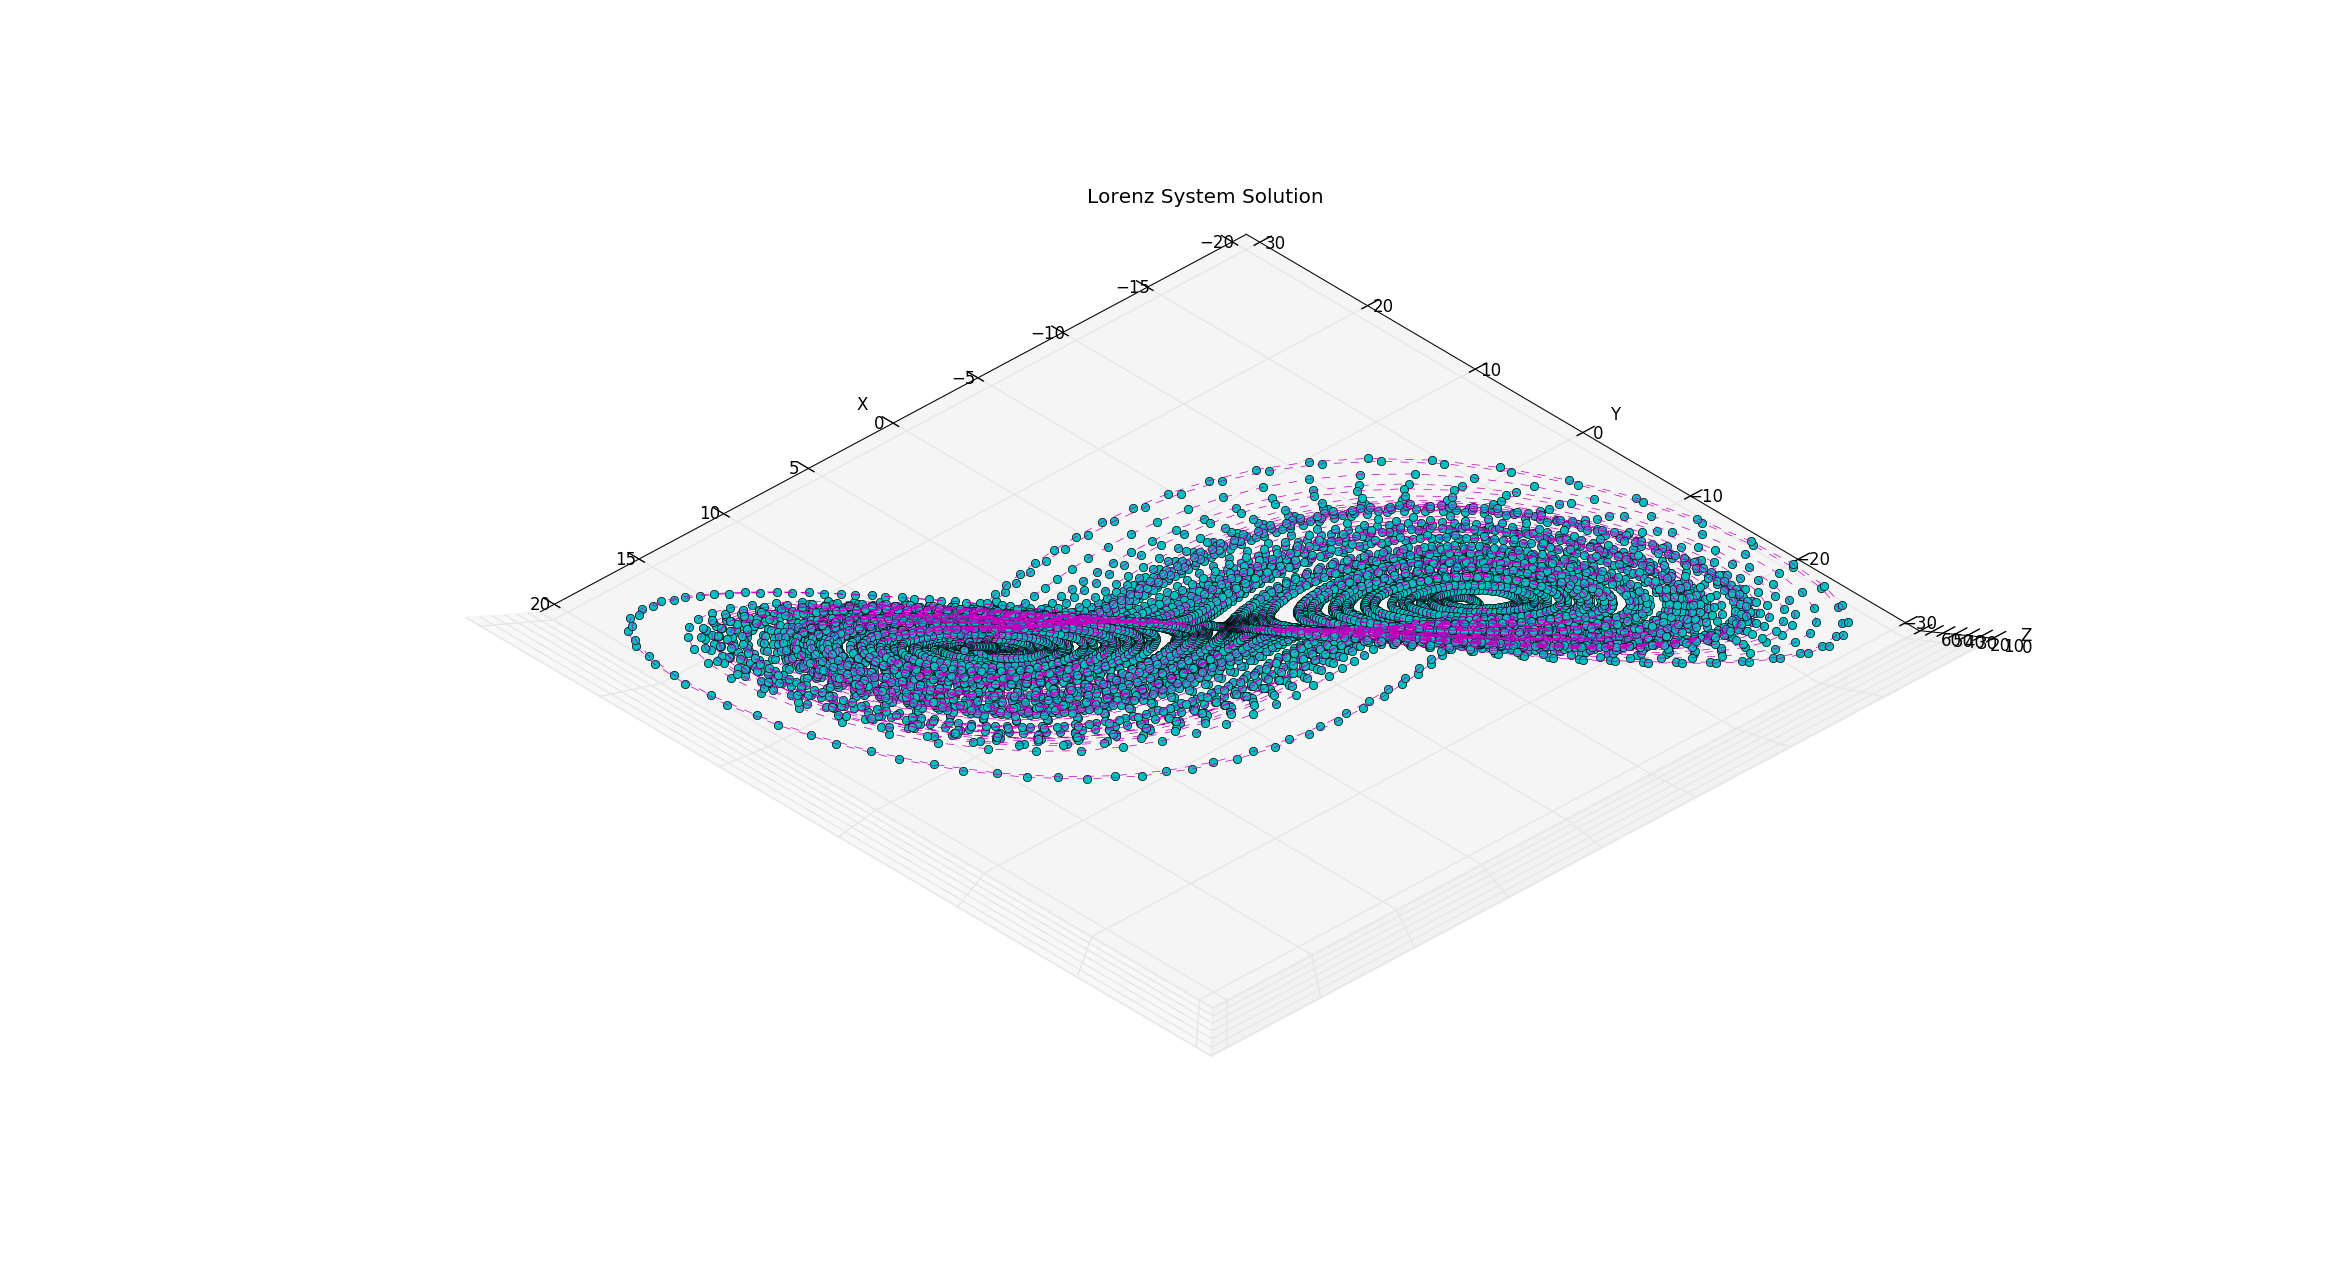
\includegraphics[width=1\linewidth, height=10cm]{q5_1.png} 
        \caption{ Upper Orientation }
        \label{fig:subim1}
    \end{subfigure}
    \begin{subfigure}{\textwidth}
        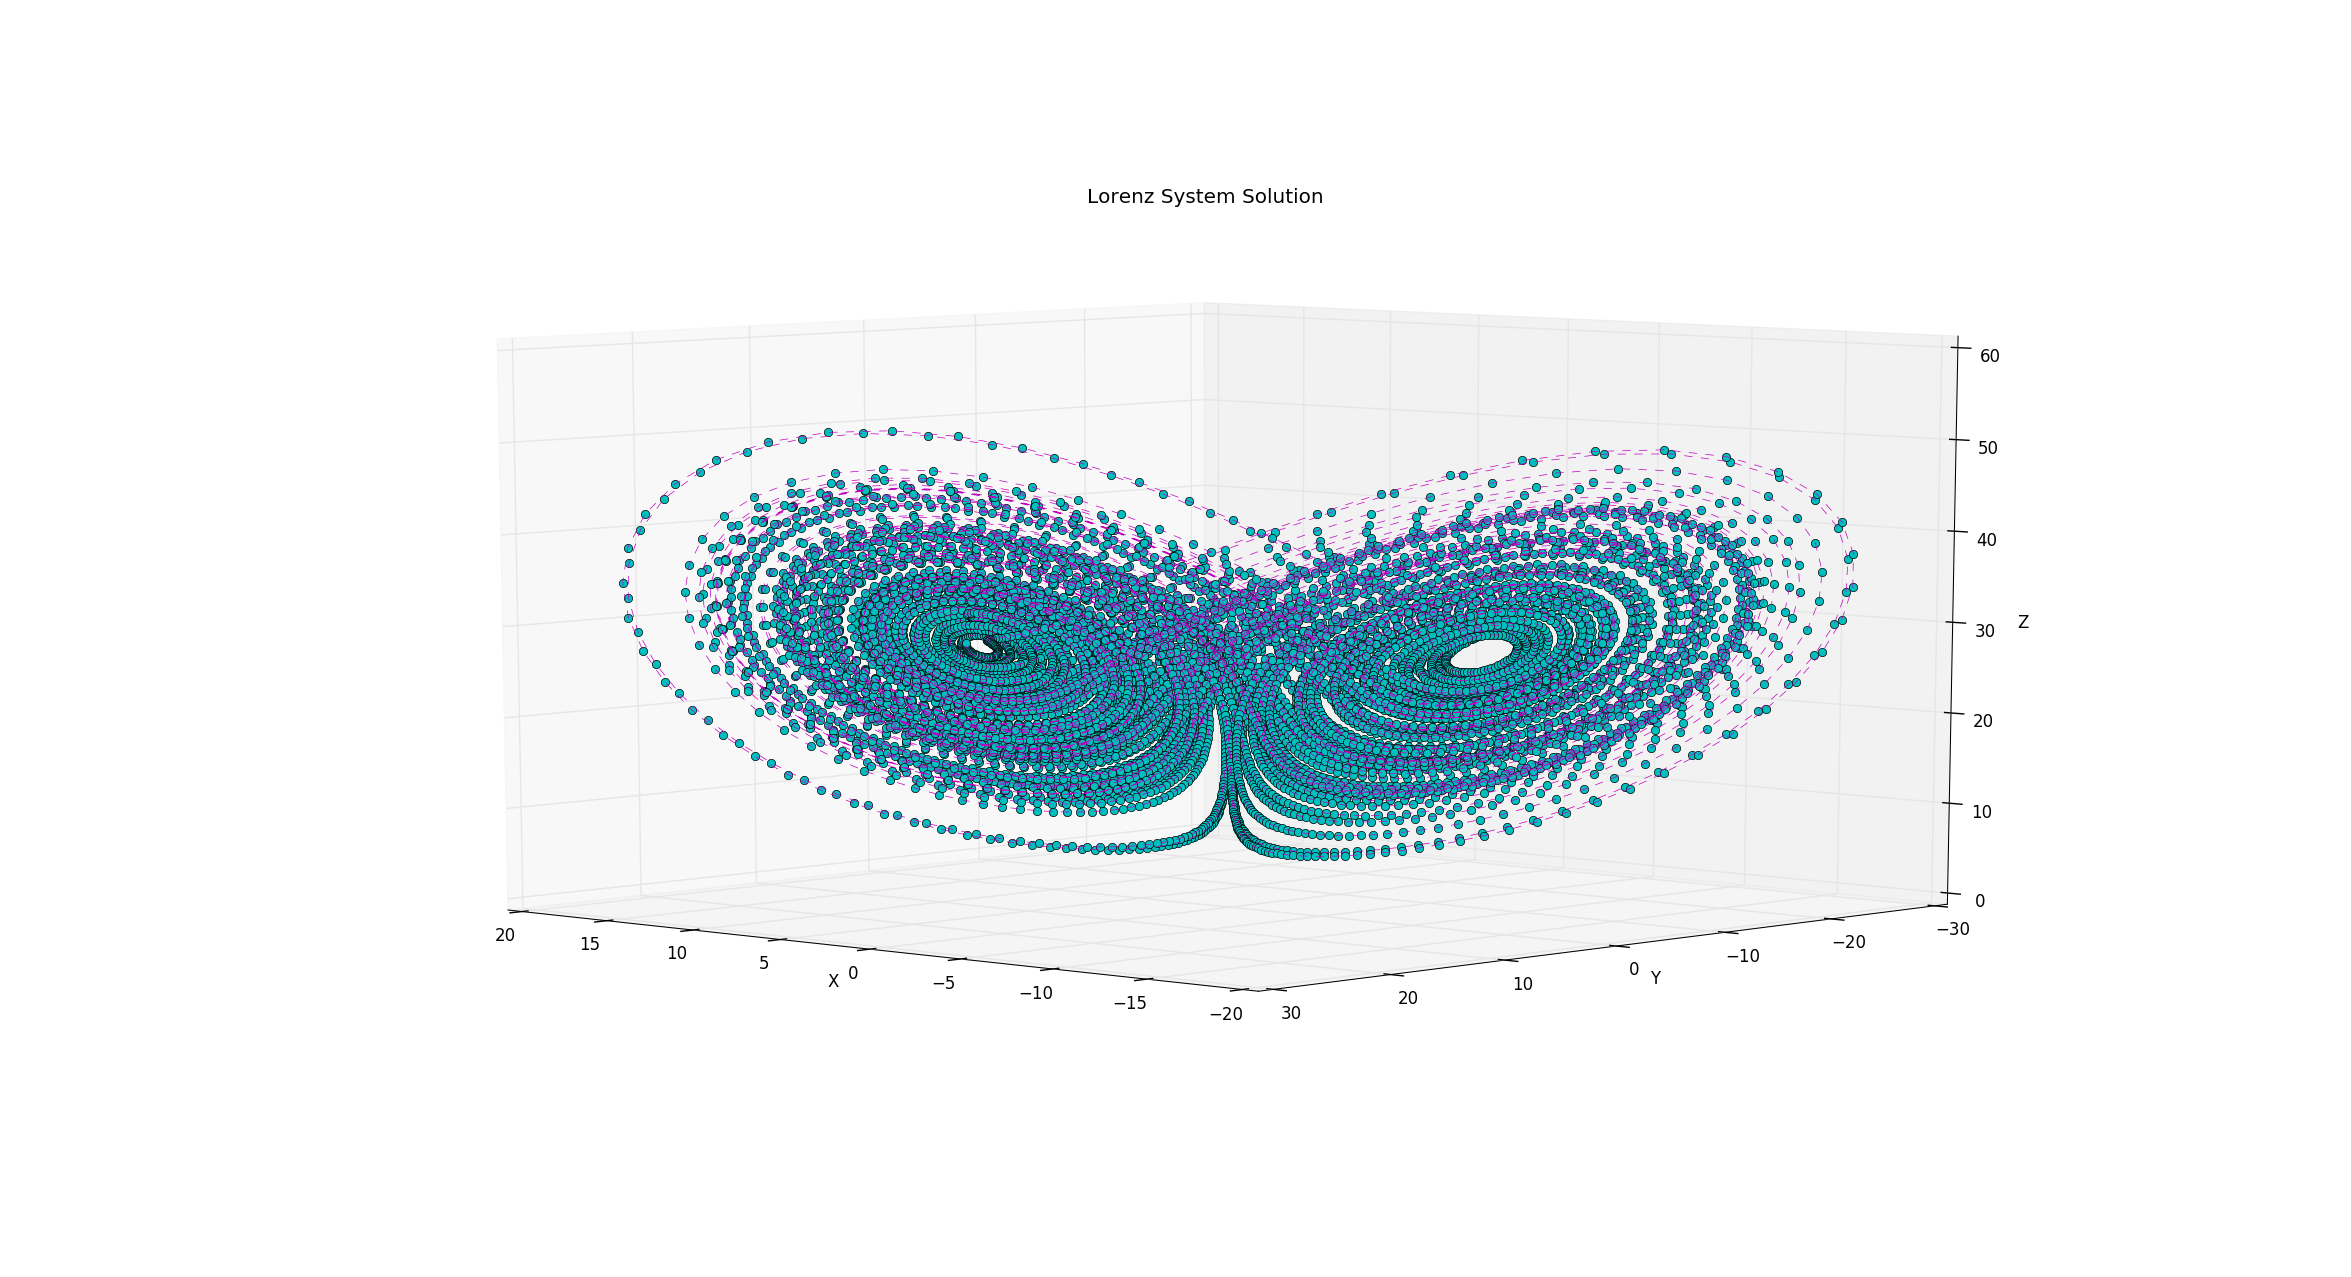
\includegraphics[width=1\linewidth, height=10cm]{q5_2.png} 
        \caption{ X-Y-Z Orientation }
        \label{fig:subim1}
    \end{subfigure}
\caption{The Lorenz Solution Diagram with the two unique views, Upper View and X-Y-Z view respectively }
\label{fig:image2}
\end{figure}
\end{center}

\end{document}